\section{Windfall of malice}

In the previous section we experienced the havoc a malicious player is capable of causing in a congestion game.
But is the opposite possible -- that there is an improvement by the malicious player?
After all, there are many paradoxes of this kind in game theory.
In this section we will see that there is indeed a \emph{Windfall of Malice}, but first we will take a look at \emph{Breass' paradox} to construct, and understand the nature of, that paradox.

\subsection{Braess' paradox}

\begin{marginfigure}
	\begin{tikzpicture}[scale=0.7]
	\SetGraphUnit{2}
	\GraphInit[vstyle=Normal]
	\SetUpEdge[style={->, thick}, color=gray]
	\tikzset{LabelStyle/.style = {fill=none, sloped, above}}
	
	% Knoten
	\Vertices[unit=3]{circle}{t,p,s,q}
	
	% Kanten
	\Edge[label=$x/2$](s)(p)
	\Edge[label=$x/2$](q)(t)
	\Edge[label=$1$](s)(q)
	\Edge[label=$1$](p)(t)
	\end{tikzpicture}
	\caption{Congestion game $\mathcal A$ with flow value $v=1$}
	\label{braess-base}
\end{marginfigure}

Braess' paradox was discovered by Dietrich Braess in 1968 and demonstrates how an additional strategic option is able to cause a worse stable solution in a congestion game than before.
In figure \ref{braess-base} we see the congestion game $\mathcal A$ with flow value $v=1$.
Because of its symmetry, the nash flow is divided in two equal parts -- on the upper path flows 1/2 and on the lower one, too.
The resulting nash delay is thus 1.25.
In the real world, we could interpret this game as a street network where daily people commute from $s$ to $t$ and the nash delay is the length of a traffic jam.

\begin{marginfigure}
	\begin{tikzpicture}[scale=0.7]
	\SetGraphUnit{2}
	\GraphInit[vstyle=Normal]
	\SetUpEdge[style={->, thick}, color=gray]
	\tikzset{LabelStyle/.style = {fill=none, sloped, above}}
	
	% Knoten
	\Vertices[unit=3]{circle}{t,p,s,q}
	
	% Kanten
	\Edge[label=$x/2$](s)(p)
	\Edge[label=$x/2$](q)(t)
	\Edge[label=$1$](s)(q)
	\Edge[label=$1$](p)(t)
	% Abkürzung
	\Edge[label=$x/2$](p)(q)
	\end{tikzpicture}
	\caption{adding the short cut ($\mathcal B$)}
	\label{braess-complete}
\end{marginfigure}

If the city council however decides to add an additional road between $p$ and $q$ (see figure \ref{braess-complete}) to decrease the congestion, they achieve the opposite -- the nash delay increases because nash flow only uses the path $s,p,q,t$.
But why?
Because the delay of the upper and of the lower path are always bigger than the delay of the central path:
Let $P$ be the upper path $s,p,t$ and $P^*$ the central path $s,p,q,t$.
Because the flow value is $v=1$ the load of an edge cannot exceed 1.
\begin{align*}
	L(P) = f(s,p)/2 + 1 \geq f(s,p)/2 + f(p,q)/2 + f(q,t)/2 = L(P^*) 
\end{align*}
By symmetry this also holds for the lower path.
And because the old nash flow is not stable any more, the only nash flow is that one which concentrates all on $P^*$.
But the nash delay is here $L(P^*) = 1.5$.

\begin{marginfigure}
	\begin{tikzpicture}[scale=0.7]
	\SetGraphUnit{2}
	\GraphInit[vstyle=Normal]
	\SetUpEdge[style={->, thick}, color=gray]
	\tikzset{LabelStyle/.style = {fill=none, sloped, above}}
	
	% Knoten
	\Vertices[unit=3]{circle}{t,p,s,q}
	
	% Kanten
	\Edge[label=$x/2$](s)(p)
	\Edge[label=$x/2$](q)(t)
	\Edge[label=$1$](s)(q)
	\Edge[label=$1$](p)(t)
	
	%innen
	\EA[Lpos=180](s){m}
	\EA[unit=2](m){n}
	\Edge[label=$0$](p)(n)
	\Edge[label=$0$](m)(n)
	\Edge[label=$0$](m)(q)
	\Edge[label=$x$](p)(m)
	\Edge[label=$x$](n)(q)
	\end{tikzpicture}
	\caption{Modified network $\mathcal C$ which has also a nash delay of 1.5}
	\label{braess-modified}
\end{marginfigure}

But before we are able to proceed to the windfall of malice we have to make a small adjustment of the congestion game above.
We replace the edge $(p,q)$ with a slightly more complex subgraph (see figure \ref{braess-modified}). 
But this subgraph behaves exactly like the edge:
Let there be a nash flow with flow value $u$ between $p$ and $q$.
Then it is divided equally between the path $p,m,q$ and $p,n,q$ and thus has a nash delay of $u/2$ -- exactly like a nash flow between $p$ and $q$ in the old network $\mathcal B$.

\subsection{Reverting Braess' paradox with the malicious player}

\begin{marginfigure}
	\begin{tikzpicture}[scale=0.7]
	\SetGraphUnit{2}
	\GraphInit[vstyle=Normal]
	\SetUpEdge[style={->, thick}, color=gray]
	\tikzset{LabelStyle/.style = {fill=none, sloped, above}}
	
	% Knoten
	\Vertices[unit=3]{circle}{t,p,s,q}
	\EA[Lpos=180](s){m}
	\EA[unit=2](m){n}
	
	% Kanten
	\Edge[label=$1$](p)(t)
	\Edge[label=$0$](p)(n)
	\SetUpEdge[style={->, thick}, color=myRed]
	\tikzset{LabelStyle/.style = {fill=none, sloped, above}}
	\Edge[label=$x/2$](s)(p)
	\Edge[label=$x$](p)(m)
	\Edge[label=$0$](m)(n)
	
	\SetUpEdge[style={->, thick}, color=gray]
	\tikzset{LabelStyle/.style = {fill=none, sloped, below}}
	\Edge[label=$1$](s)(q)
	\Edge[label=$0$](m)(q)
	\SetUpEdge[style={->, thick}, color=myRed]
	\tikzset{LabelStyle/.style = {fill=none, sloped, below}}
	\Edge[label=$x$](n)(q)
	\Edge[label=$x/2$](q)(t)
	\end{tikzpicture}
	\caption{Game $\mathcal C$ with a malicious player's \textsc{Mbr} drawn in with red colour.}
	\label{wof-mbr}
\end{marginfigure} 

After discussing Braess' paradox we address the windfall of malice.
What happens if we add a malicious player to the game $\mathcal C$ from above?
We see a \emph{decrease} of the nash delay!
In some manner, the windfall of malice counteracts Braess' paradox.

To analysis this behaviour, we first determine the malicious best response.
The \textsc{Mbr} is always the path $s,p,m,n,q,t$ because it covers all edges with non-constant latency functions (similar like in the section before).
\begin{marginfigure}
	\begin{tikzpicture}[scale=0.7]
	\SetGraphUnit{2}
	\GraphInit[vstyle=Normal]
	\SetUpEdge[style={->, thick}, color=gray]
	\tikzset{LabelStyle/.style = {fill=none, sloped, above}}
	
	% Knoten
	\Vertices[unit=3]{circle}{t,p,s,q}
	
	% Kanten
	\Edge[label=$1$](p)(t)
	\Edge[label=$(x+w)/2$](s)(p)
	
	\SetUpEdge[style={->, thick}, color=gray]
	\tikzset{LabelStyle/.style = {fill=none, sloped, below}}
	\Edge[label=$1$](s)(q)
	\Edge[label=$(x+w)/2$](q)(t)
	\SetUpEdge[style={->, dashed, thick}, color=gray]
	\tikzset{LabelStyle/.style = {fill=none, sloped, above}}
	\Edge[label=$x/2 + w$](p)(q)
	\end{tikzpicture}
	\caption{Induced game with $w$ malicious flow value and where the subgraph between $p$ and $q$ is contracted / simplified. Observe, that the latency function on $(p,q)$ is strictly larger than on $(s,p)$ and $(q,t)$.}
	\label{wof-induced-simplified}
\end{marginfigure}
In figure \ref{wof-induced-simplified} we see the induced (and simplified) game $\mathcal C^g$ by the \textsc{Mbr}.
If the malicious flow value is $w=0$ nothing changes, but else the higher $w$ gets the more of the nash flow is split up to the upper and lower path.
\begin{lemma}
	If we add a malicious player with flow value $w$ to the game $\mathcal C$, then the old nash flow ($f(P^*)=1-w$, else $f(P)=0$ with $P^*=(s,p,q,t)$) is \emph{not} part of the nash equilibrium in $\mathcal C$.
\end{lemma}

\begin{proof}
	Let the malicious flow $g$ be the \textsc{Mbr} with malicious flow value $w > 0$ and $f$ the old nash flow (see the lemma).
	Then the latency on the path $P^*$ is 
	\[L(P^*) = (1-w+w)/2 + (1-w)/2 + w + (1-w+w)/2 = 1.5 + w/2 .\]
	But this latency is greater than the one of the upper path $P'=(s,p,t)$ : $L(P')= (1-w+w)/2 + 1 = 1.5$.
	Thus $f$ is not a nash flow and $(f,g)$ is not a nash equilibrium.
\end{proof}

With the same proof idea we follow this
\begin{corollary}
	If the malicious flow value $w$ is strictly larger than 2/3, Braess' paradox is completely reversed:
	The nash delay is 1.25 and nash equilibrium is $(f,g)$ where $f$ is the nash flow from $\mathcal A$ and $g$ is the \textsc{Mbr} to $f$. 
\end{corollary}
